\documentclass{article}

\usepackage[left=2cm,right=2cm, top=2cm, bottom = 2cm]{geometry}
\usepackage{amsfonts}
\usepackage{amsmath}
\usepackage{array}
\usepackage{tikz}

\setlength{\tabcolsep}{1.8cm}
\renewcommand{\arraystretch}{2.5}

\makeatletter
\newcommand{\thickhline}{%
    \noalign {\ifnum 0=`}\fi \hrule height 2pt
    \futurelet \reserved@a \@xhline
}
\newcolumntype{!}{@{\hskip\tabcolsep\vrule width 2pt\hskip\tabcolsep}}
\makeatother

\begin{document}

\title{Trigonometry--Summary}
\date{}

\maketitle
\thispagestyle{empty}
\pagestyle{empty}

\Large

\section{Key Points - Fill in the Blanks:}

Fill in the blanks in the key points below with a word or phrase. The unblanked versions are on the next page. Bear in mind that in some cases there may be several ways to phrase things, so if what you put isn't exactly what I had, that doesn't mean it's necessarily wrong. Ask for any clarification! Note that the size of the blank does not indicate the size of the missing word or phrase!

\begin{enumerate}
\item In a right-angled triangle with an angle $\theta$, we call the three sides the ..............., the ..............., and the ................
\item In a right-angled triangle with an angle $\theta$, we can express the trigonometric functions as ratios of the sides:
	\[\sin(\theta)=\frac{\cdot}{\cdot}\qquad \cos(\theta)=\frac{\cdot}{\cdot}\qquad \tan(\theta)=\frac{\cdot}{\cdot}\]
\item To define the trigonometric functions for arbitrary angles, we take the point on the ......... circle at an angle $\theta$ from ................ and define $\sin(\theta)$ to be the ....-	coordinate and $\cos(\theta)$ to be the ....-coordinate of that point.
\item Tangent is related to sine and cosine by the equation:
	\[\tan(\theta) = ...\]
\item The \textbf{pythagorean equation} for sine and cosine is .....
\item The $(x,y)$-coordinates of a point are called its ......... coordinates. The $(r,\theta)$-coordinates are called ......... coordinates. To convert between them, we use the equations:
	\[x=...\qquad y=...\]
	\[r=...\qquad \tan(\theta)=...\]
\item A \textbf{sinusoid} is any curve obtained from the sine wave by applying a ......
\item Given the graph of $y=f(x)$, to obtain the graph of:
	\begin{enumerate}
		\item $y=f(x)+a$ we translate upwards by $a$.
		\item $y=f(x+a)$ we .....
		\item $y=af(x)$ we ....
		\item $y=f(ax)$ we .....
	\end{enumerate}
\item The \textit{compound angle formulae} are:
	\[\sin(\alpha+\beta)=...\]
	\[\cos(\alpha+\beta)=...\]
	\[\tan(\alpha+\beta)=...\]
\item We can convert a product of two sines or of two cosines into a sum of cosines by the formulae:
	\[\cos(\alpha)\cos(\beta)=...\]
	\[\sin(\alpha)\sin(\beta)=...\]
\item A sum of sinusoids \textbf{of the same frequency} is a .....
\item A sum of sinusoids of different frequencies, or a product of sinusoids, is a .......
\end{enumerate}

\clearpage

\section{Key Points to Remember}

The statements from the previous page, with the blanks filled in.

\begin{enumerate}
\item In a right-angled triangle with an angle $\theta$, we call the three sides the \textit{opposite}, the \textit{adjacent}, and the \textit{hypotenuse}.
\item In a right-angled triangle with an angle $\theta$, we can express the trigonometric functions as ratios of the sides:
	\[\sin(\theta)=\frac{\mathrm{opposite}}{\mathrm{hypotenuse}}\qquad \cos(\theta)=\frac{\mathrm{adjacent}}{\mathrm{hypotenuse}}\qquad \tan(\theta)=\frac{\mathrm{opposite}}		{\mathrm{adjacent}}\]
\item To define the trigonometric functions for arbitrary angles, we take the point on the \textit{unit} circle at an angle $\theta$ from \textit{the positive $x$-axis} and define $\sin(\theta)$ to be the $y$-coordinate and $\cos(\theta)$ to be the $x$-coordinate of that point.
\item Tangent is related to sine and cosine by the equation:
	\[\tan(\theta) = \frac{\sin(\theta)}{\cos(\theta)}.\]
\item The \textbf{pythagorean equation} for sine and cosine is
	\[\sin^2(\theta)+\cos^2(\theta)=1\]
\item The $(x,y)$-coordinates of a point are called its \textit{cartesian} (or \textit{rectangular}) coordinates. The $(r,\theta)$-coordinates are called \textit{(plane) polar} coordinates. To convert between them, we use the equations:
	\[x=r\cos(\theta)\qquad y=r\sin(\theta)\]
	\[r=\sqrt{x^2+y^2}\qquad \tan(\theta)=\frac{y}{x}\]
\item A \textbf{sinusoid} is any curve obtained from the sine wave by applying a \textit{location-scale transformation}.
\item Given the graph of $y=f(x)$, to obtain the graph of:
	\begin{enumerate}
		\item $y=f(x)+a$ we translate upwards by $a$.
		\item $y=f(x+a)$ we \textit{translate to the left by $a$}.
		\item $y=af(x)$ we \textit{stretch vertically by a factor of $a$}.
		\item $y=f(ax)$ we \textit{squash horizontally by a factor of $a$}.
	\end{enumerate}
\item The \textit{compound angle formulae} are:
	\[\sin(\alpha+\beta)=\sin(\alpha)\cos(\beta)+\cos(\alpha)\sin(\beta)\]
	\[\cos(\alpha+\beta)=\cos(\alpha)\cos(\beta)-\sin(\alpha)\sin(\beta)\]
	\[\tan(\alpha+\beta)=\frac{\tan(\alpha)+\tan(\beta)}{1-\tan(\alpha)\tan(\beta)}\]
\item We can convert a product of two sines or of two cosines into a sum of cosines by the formulae:
	\[\cos(\alpha)\cos(\beta)=\frac{1}{2}\left(\cos(\alpha+\beta)+\cos(\alpha-\beta)\right)\]
	\[\sin(\alpha)\sin(\beta)=\frac{1}{2}\left(\cos(\alpha-\beta)-\cos(\alpha+\beta)\right)\]
\item A sum of sinusoids \textbf{of the same frequency} is a \textit{sinusoid}.
\item A sum of sinusoids of different frequencies, or a product of sinusoids, is a \textit{more complicated waveform}.
\end{enumerate}


\clearpage

\section{Revision Questions}

\begin{enumerate}
\item Convert the following points from cartesian coordinates to polar coordinates:
	\begin{enumerate}
	\item $(0,-3)$
	\item $(4,3)$
	\item $(-1,7)$
	\end{enumerate}
\item Convert the following points from polar coordinates to cartesian coordinates:
	\begin{enumerate}
	\item $(13,0)$
	\item $\left(2,\frac{\pi}{3}\right)$
	\item $\left(9,\frac{9\pi}{8}\right)$
	\end{enumerate}
\item Suppose $\sin(\alpha)=\frac{1}{2}$ and $\sin(\beta)=\frac{1}{\sqrt{2}}$, and that $\alpha$ lies in the top right-hand quadrant, while $\beta$ lies in the top left-hand quadrant.
	\begin{enumerate}
	\item Compute $\cos(\alpha-\beta)$ \textit{without finding $\alpha$ or $\beta$}.
	\item What are $\alpha$ and $\beta$?
	\end{enumerate}
\item Below is shown the graph of a function, $y=f(x)$. Sketch the graphs of
	\begin{enumerate}
	\item $y=f(x-1)+2$
	\item $y=2f(x)$
	\item $y=f\left(\frac{x}{2}\right)$.
	\end{enumerate}
\item Write $\sin(5t)\sin(\pi t)$ as a sum of sinusoids.
\item Write $12\cos(t)-5\sin(t)$ in the form $R\cos(t+\alpha)$.
\item Write $8\cos(\pi t) + 8\cos(\pi(t+1))$ in the form $R\sin(\pi t+\alpha)$.	
\end{enumerate}

\begin{center}
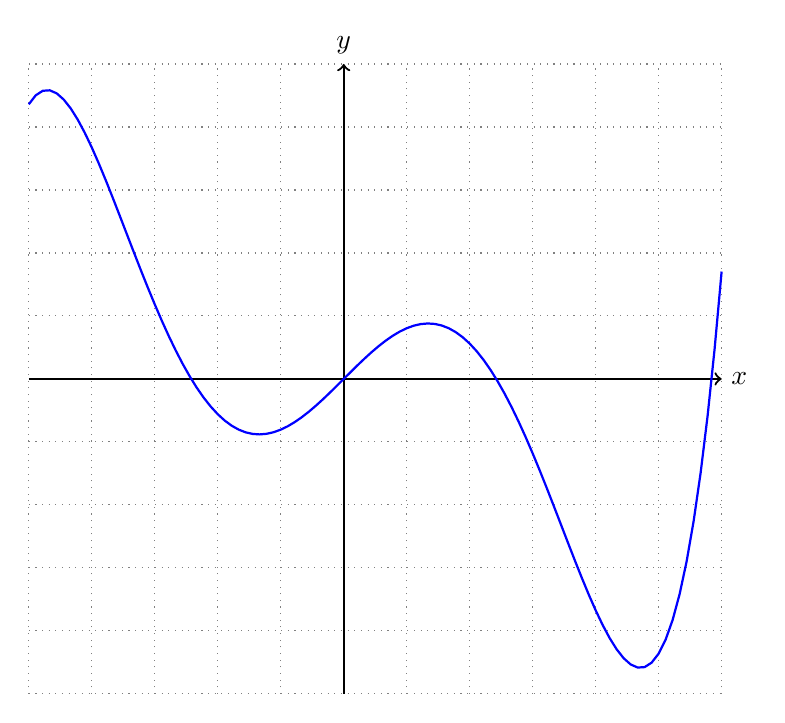
\begin{tikzpicture}[scale=0.8]
\draw[dotted,gray] (-5,-5) grid (6,5);
\draw[thick,->] (-5,0) -- (6,0);
\node[right] at (6,0) {$x$};
\draw[thick,->] (0,-5) -- (0,5);
\node[above] at (0,5) {$y$};

\draw[blue,thick, domain=-5:6, samples=100] plot (\x,{ (0.005*\x^5)-(0.2*\x^3)+(\x) });
\end{tikzpicture}
\end{center}



\clearpage

\section{Solutions}

It is possible I've made a mistake or two in these, so if your answer is different from mine and after checking you can't find a mistake in your work, ask me about it!

\begin{enumerate}
\item 
	\begin{enumerate}
	\item $\left(3,\frac{3\pi}{2}\right)$
	\item $(5,0.927)$
	\item $(7.07,1.713)$
	\end{enumerate}
\item
	\begin{enumerate}
	\item $(13,0)$
	\item $(1,\sqrt{3})\approx(1,1.732)$
	\item $(-8.315,-3.444)$
	\end{enumerate}
\item
	\begin{enumerate}
	\item From the pythagorean identity, $\cos^2(\alpha)=1-\left(\frac{1}{2}\right)^2=\frac{3}{4}$, and $\alpha$ is in the first quadrant, so $\cos(\alpha)>0$; therefore $\cos(\alpha)=\frac{\sqrt{3}}{2}$. Similarly, $\cos^2(\beta)=1-\frac{1}{2}=\frac{1}{2}$ and $\cos(\beta)<0$, so $\cos(\beta)=\frac{-1}{\sqrt{2}}$. So
	\[\cos(\alpha-\beta)=\cos(\alpha)\cos(\beta)+\sin(\alpha)\sin(\beta)=\frac{\sqrt{3}}{2}\times\frac{-1}{\sqrt{2}}+\frac{1}{2}\times\frac{1}{\sqrt{2}}=\frac{1-\sqrt{3}}{2\sqrt{2}}\]
	\item \[\alpha=\sin^{-1}\left(\frac{1}{2}\right) = \frac{\pi}{6}\qquad \beta=\sin^{-1}\left(\frac{1}{\sqrt{2}}\right)=\frac{\pi}{4}.\]
	\end{enumerate}
\item See graphs below.
\item
	\[\sin(5t)\sin(\pi t)=\frac{1}{2}\left(\cos((5-\pi)t)-\cos((5+\pi)t)\right)\]
\item
	\begin{align*}
	12\cos(t)-5\sin(t)&=R\cos(t+\alpha)\\
	&=R\cos(t)\cos(\alpha)-R\sin(t)\sin(\alpha)
	\end{align*}
	So $R\cos(\alpha)=12$, and $R\sin(\alpha)=-5$. Therefore $R^2=12^2+5^2=169=13^2$, so $R=13$, and
	\[\tan(\alpha)=\frac{-5}{12}.\]
	Since $\sin(\alpha)<0$ and $\cos(\alpha)>0$, we are in the bottom-right quadrant, so $\alpha=\tan^{-1}\left(\frac{-5}{12}\right)\approx-0.395$. So
	\[12\cos(t)-5\sin(t)=13\cos(t-0.395).\]
\item
	\begin{align*}
	8\cos(\pi t) + 8\cos(\pi(t+1))&=8\cos(\pi t) + 8(\cos(\pi t)\cos(\pi)-\sin(\pi t)\sin(\pi))\\
	&= 8\cos(\pi t) -8\cos(\pi t) - 0\\
	&= 0
	\end{align*}
	So in fact these sinusoids cancel out exactly! The result is the zero wave, which can be thought of as a sinusoid with amplitude 0.
\end{enumerate}


\begin{center}
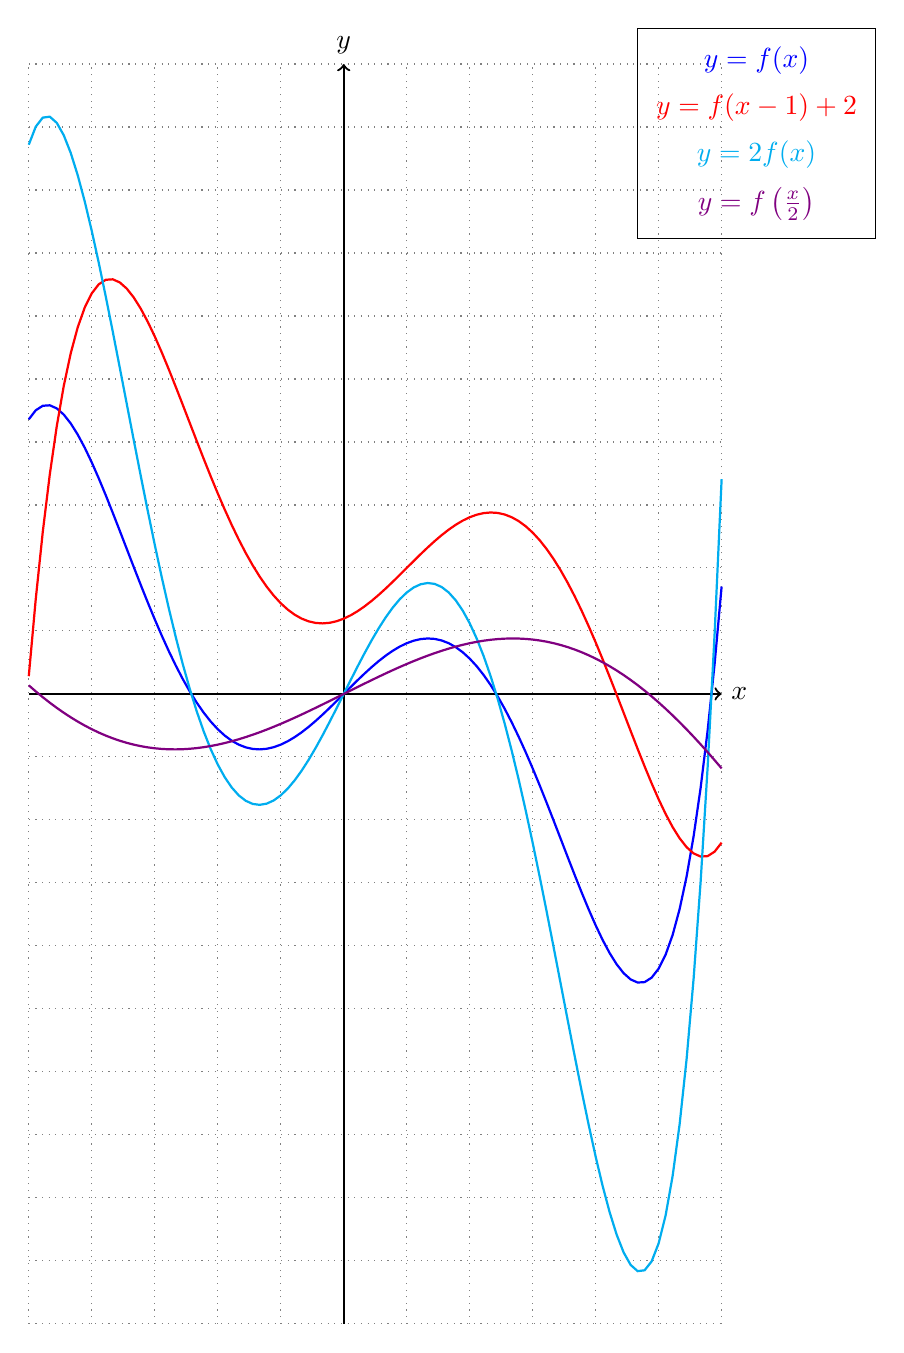
\begin{tikzpicture}[scale=0.8]
\draw[dotted,gray] (-5,-10) grid (6,10);
\draw[thick,->] (-5,0) -- (6,0);
\node[right] at (6,0) {$x$};
\draw[thick,->] (0,-10) -- (0,10);
\node[above] at (0,10) {$y$};

\draw[blue,thick, domain=-5:6, samples=100] plot (\x,{ (0.005*\x^5)-(0.2*\x^3)+(\x) });
\draw[red,thick, domain=-5:6, samples=100] plot (\x,{ (0.005*(\x-1)^5)-(0.2*(\x-1)^3)+(\x-1)+2 });
\draw[cyan,thick, domain=-5:6, samples=100] plot (\x,{ 2*((0.005*(\x)^5)-(0.2*(\x)^3)+(\x)) });
\draw[violet,thick, domain=-5:6, samples=100] plot (\x,{ (0.005*(\x/2)^5)-(0.2*(\x/2)^3)+(\x/2) });

\matrix [draw,below] at (current bounding box.north east) {
	\node [blue] {$y=f(x)$}; \\
	\node [red] {$y=f(x-1)+2$}; \\
	\node[cyan] {$y=2f(x)$};\\
	\node[violet] {$y=f\left(\frac{x}{2}\right)$};\\
};
\end{tikzpicture}
\end{center}

\clearpage



\section{Key Formulae to Remember}

\vspace{5mm}

Note: I am a firm believer that rote memorisation is rarely a good idea and should have only a very limited place in maths education. To be good at English, you need to know the definitions of thousands of words, but no one suggests getting English students to memorise definitions, after all! Words are learnt by using them; similarly, mathematical formulae are best learnt by using them, and understanding where they come from.

The way I learned those formulae I know is by using them a lot; typically I have to look them up the first few dozen times. After I've used them enough, I find they stick in my memory. Understanding how they are derived and how they link to other mathematical concepts is also useful for helping to remember them.

So you're free to do what you want with this list, and if you want to try learning them by rote, feel free, but I would strongly encourage you to use this instead as a reference list for practising with them!

\begin{enumerate}
\item \[\sin^2(\theta)+\cos^2(\theta)=1\]
\item \[\sin(\alpha+\beta)=\sin(\alpha)\cos(\beta)+\cos(\alpha)\sin(\beta)\]
\item \[\cos(\alpha+\beta)=\cos(\alpha)\cos(\beta)-\sin(\alpha)\sin(\beta)\]
\item Converting from polars to cartesians:
	\[x=r\cos(\theta)\qquad y=r\sin(\theta)\]
\item Converting from catesians to polars:
	\[r=\sqrt{x^2+y^2}\qquad \tan(\theta)=\frac{y}{x}\]
	and check the quadrant to determine whether or not to add $\pi$ to $\tan^{-1}\left(\frac{y}{x}\right)$ to get $\theta$.
\item \[\cos(\alpha)\cos(\beta)=\frac{1}{2}[\cos(\alpha+\beta)+\cos(\alpha-\beta)]\]
\item \[\sin(\alpha)\sin(\beta)=\frac{1}{2}[\cos(\alpha-\beta)-\cos(\alpha+\beta)\]
\end{enumerate}




\end{document}